H-graphs shown in Figure \ref{fig:H-graph} are the simplest graphs which are not such graphs.
It is expected that H-graphs yield non-Siefert manifolds.
\begin{figure}[h]	\centering
		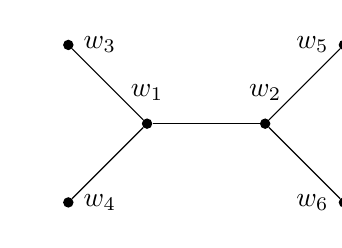
\begin{tikzpicture}
			\node[shape=circle,fill=black, scale = 0.4] (1) at (0,0) { };
			\node[shape=circle,fill=black, scale = 0.4] (2) at (1.5,0) { };
			\node[shape=circle,fill=black, scale = 0.4] (3) at (-1,-1) { };
			\node[shape=circle,fill=black, scale = 0.4] (4) at (-1,1) { };
			\node[shape=circle,fill=black, scale = 0.4] (5) at (2.5,1) { };
			\node[shape=circle,fill=black, scale = 0.4] (6) at (2.5,-1) { };
			
			\node[draw=none] (B1) at (0,0.4) {$ w_1 $};
			\node[draw=none] (B2) at (1.5, 0.4) {$ w_2 $};
			\node[draw=none] (B3) at (-0.6,1) {$ w_3 $};
			\node[draw=none] (B4) at (-0.6,-1) {$ w_4 $};
			\node[draw=none] (B5) at (2.1,1) {$ w_5 $};		
			\node[draw=none] (B6) at (2.1,-1) {$ w_6 $};	
			
			\path [-](1) edge node[left] {} (2);
			\path [-](1) edge node[left] {} (3);
			\path [-](1) edge node[left] {} (4);
			\path [-](2) edge node[left] {} (5);
			\path [-](2) edge node[left] {} (6);
		\end{tikzpicture}
		\caption{The H-graph $ \Gamma $.}\label{fig:H-graph}
	\end{figure}

In the case of H-graphs, Bringmann--Mahlburg--Milas~\cite{BMM} showed that radial limits of homological blocks coincide with sums of radial limits of multiple Eichler integrals.
Moreover, they proved that the radial limits of a homological block make up a quantum modular form of depth two and of weight one with the quantum set $ \mathbb{Q} $.

Meanwhile, for non-Seifert manifolds, it remains to be seen whether WRT invariants relate to homological blocks \cite[Conjecture~2.1]{GPPV} and have modularity.

In this paper, we study WRT invariants of H-graphs.
We will write them explicitly as weighted Gauss sums.
Moreover, we will prove that they relate to homological blocks and they yield quantum modular forms of depth two and of weight one with the quantum set $ \mathbb{Q} $.

Let us explain our setting.
Let $ \Gamma $ be the H-graph with vertices $ 1, \dots, 6 $ and weights $ w_v \in \Z_{<0} $ for each vertex $ v $ shown in Figure~\ref{fig:H-graph} such that its linking matrix
\begin{gather*}
W = \pmat{w_1 & 1 & 1 & 1 & 0 & 0 \\
	1 & w_2 & 0 & 0 & 1 & 1 \\
	1 & 0 & w_3 & 0 & 0 & 0 \\
	1 & 0 & 0 & w_4 & 0 & 0 \\
	0 & 1 & 0 & 0 & w_5 & 0 \\
	0 & 1 & 0 & 0 & 0 & w_6 }
\end{gather*}
is negative definite and its determinant is $ 1 $.


Then we obtain the link $ \calL(\Gamma) $ defined by $ \Gamma $ shown in Figure \ref{fig:surgery_diagram}.
Let $M_3(\Gamma)$ be the plumed 3-ma\-nifold obtained from $ S^3 $ through the surgery along the diagram $ \calL(\Gamma) $.
We obtain $H_1(M_{3}(\Gamma), \Z)\allowbreak \cong \Z^{6} / W\big(\Z^{6}\big)$ by use of the Mayer--Vietoris sequence.
Since $\det W = 1$, $M_{3}(\Gamma)$ is an integral homology sphere.
\begin{figure}[h]	\centering
\begin{tikzpicture}[scale=0.5]
			\begin{knot}[
				clip width=5,
				flip crossing=2,
				flip crossing=4,
				flip crossing=6,
				flip crossing=7,
				flip crossing=9
				]
				\strand[thick] (0, 0) circle [x radius=3cm, y radius=1.5cm];
				\strand[thick] (0, 0) +(4cm, 0pt) circle [x radius=3cm, y radius=1.5cm];
				\strand[thick] (0, 0) +(-2.5cm, 2cm) circle [radius=1.5cm];
				\strand[thick] (0, 0) +(-2.5cm, -2cm) circle [radius=1.5cm];
				\strand[thick] (0, 0) +(6.5cm, 2cm) circle [radius=1.5cm];
				\strand[thick] (0, 0) +(6.5cm, -2cm) circle [radius=1.5cm];
				
				\node (1) at (0, 2) {$w_{1}$};
				\node (2) at (4, 2) {$w_{2}$};
				\node (3) at (-2.5, 4) {$w_{3}$};
				\node (4) at (-2.5, -4) {$w_{4}$};
				\node (5) at (6.5, 4) {$w_{5}$};
				\node (6) at (6.5, -4) {$w_{6}$};
			\end{knot}
		\end{tikzpicture}
\caption{The surgery diagram $ \calL(\Gamma) $ corresponding to $\Gamma$.}\label{fig:surgery_diagram}
\end{figure}

{\samepage
Such H-graphs yield Seifert manifolds if $ w_v = -1 $ for some $ 3 \le v \le 6 $.
Bringmann--Mahlburg--Milas~\cite[Theorem~1.2]{BMM} showed that there exist precisely $ 39 $ equivalence classes of such H-graphs with $ w_v \le -2 $ for each $ 3 \le v \le 6 $ up to graph isomorphism.

}

For a positive integer $k$, let $\tau_k$ be the WRT invariant normalised as $\tau_{k}\big(S^{3}\big) = 1$.
We study a~relation between the WRT invariant $\tau_{k}(M_{3}(\Gamma))$ and the homological block $\widehat{Z}_\Gamma (q)$.

For each complex number $ z $, we denote $ \bm{e}(z) := {\rm e}^{2\pi {\rm i} z} $.
For a point $ \tau \in \bbH $, let $ q := \bm{e}(\tau) $.
Gukov--Pei--Putrov--Vafa~\cite[formula~(3.145)]{GPPV} defined the homogical block $ \widehat{Z}(q) $ of the plumed graph.
In~our case, it can be written as
\begin{gather}
\widehat{Z}_\Gamma (q)		= \widehat{Z}_{\Gamma, \delta} (q)
= \widehat{Z}_\delta (q):=
q^{(18 - w_1 - \cdots - w_6)/4} \nonumber
\\
\hphantom{\widehat{Z}_\Gamma (q)= \widehat{Z}_{\Gamma, \delta} (q) = \widehat{Z}_\delta (q):=}
{}\times \mathrm{v.p.}\int_{\abs{z_v} = 1, 1 \le v \le 6}
\frac{\big(z_3 - z_3^{-1}\big)\big(z_4 - z_4^{-1}\big)\big(z_5 - z_5^{-1}\big)\big(z_6 - z_6^{-1}\big)}{\big(z_1 - z_1^{-1}\big)\big(z_2 - z_2^{-1}\big)}\nonumber\\
\hphantom{\widehat{Z}_\Gamma (q)= \widehat{Z}_{\Gamma, \delta} (q) = \widehat{Z}_\delta (q):=}
{}\times
\Theta_{-W, \delta} (q; z_1, \dots, z_6)
 \prod_{1 \le v \le 6} \frac{{\rm d}z_v}{2\pi {\rm i} z_v},
\label{eq:homological_block_for_H}
\end{gather}
where $ \delta := \trans{(1, 1, 1, 1, 1, 1)} $ is the signature of indexes of vertices of $ \Gamma $, $ \mathrm{v.p.} $ denotes the Cauchy principal value, and
\begin{gather*}
\Theta_{-W, \delta} (q; z_1, \dots, z_6) :=
\sum_{\bm{l} = \trans{(l_1, \dots, l_6)} \in 2\Z^6 + \delta} q^{-\trans{\bm{l}} W^{-1} \bm{l}/4} \prod_{1 \le v \le 6} z_v^{l_v}
\end{gather*}
is the theta function of the linking matrix~$ W $.

\cite[Conjecture 2.1 and relation~(A.28)]{GPPV} states a conjectural relation between the WRT invariants and radial limits of the homological blocks.
In our case, their relation is
\begin{equation} \label{eq:GPPV}
	\tau_k(M_3(\Gamma)) = \frac{1}{2\big(\zeta_{2k} - \zeta_{2k}^{-1}\big)}
	\lim_{\substack{q \to \zeta_k \\
			\abs{q} < 1	}
	} \widehat{Z}_\Gamma (q),
\end{equation}
where $ \zeta_k := {\rm e}^{2\pi {\rm i}/k} $.
In this paper, we prove this relation.

\begin{Theorem} \label{thm:WRT_homological_block_main}
	The notation being as above, $(\ref{eq:GPPV})$ holds.
\end{Theorem}

The proof of Theorem \ref{thm:WRT_homological_block_main} takes several steps as below:
\begin{enumerate}\itemsep=0pt
\setlength{\leftskip}{0.45cm}
	\item[$Step~1.$]% \label{item:plan1}
We give a formula (Proposition \ref{prop:WRT_inv}) for the WRT invariant $\tau_{k}(M_{3}(\Gamma))$ analogous to the formula given by Lawrence--Rozansky~\cite[formula~(4.2)]{LR} for any Seifert fibered manifold.
	This formula involves a certain type of quadratic forms of rank two which appear in false theta functions in~\cite[Proposition 5.3]{BMM} related to the homological blocks.
	\item[$Step~2.$] %\label{item:plan2}
The sum involved in the formula (Proposition \ref{prop:WRT_inv}) is incomplete, that is, it is like a~form
	\begin{gather*}
	\sum_{n \in (\Z \smallsetminus k\Z)/kN\Z} f(n).
	\end{gather*}
	That means, we can not apply usual techniques in number theory.
	To avoid this situation, we interpolate the sum in the above formula for $\tau_{k}(M_{3}(\Gamma))$ by adding terms which diverge a priori.
	These terms turn out to be zero by vanishing results of ``weighted'' Gauss sums (Proposition \ref{prop:Gauss_sum}).
	\item[$Step~3.$] %\label{item:plan3}
In Proposition \ref{prop:Phi_lim}, we prove that the radial limit of the homological block coincides with the interpolated formula of the WRT invariant by using the Euler--Maclaurin summation formula (Lemma \ref{lem:Euler-Maclaurin}) and vanishing results of weighted Gauss sums (Proposition \ref{prop:Gauss_sum}).
\end{enumerate}
As for our formula in \emph{Step}~1, we need to handle rank two quadratic forms which do not appear in Seifert case.
In \emph{Step}~2, we need some vanishing results for Gauss sums which we develop in this article.

We need more notation to explain the next main result.
Let $ S = ( l_{jk})_{1 \le j, k \le 2} $ be the submatrix of $ -W^{-1} = (l_{jk})_{1 \le j, k \le 6} $.
Let
\begin{gather*}
Q(m, n) := (m, n) S \trans{(m, n)}, \\
M := w_3 w_4, \\
N := w_5 w_6,
\\
a := -w_2 w_5 w_6 + w_5 + w_6, \\
c := -w_1 w_3 w_4 + w_3 + w_4.
\end{gather*}
Then we have $ Q(m, n) = Mam^2 - 2MNmn + Ncn^2 $ by a direct calculation and $ S^{-1}\big(\Z^2\big) = \frac{1}{M}\Z \oplus \frac{1}{N}\Z $ by Remark~\ref{rem:S_inv_factor}.

For non-zero integers $ w $ and $ w' $, we define a map $ \chi^{(w, w')} \colon \Z \to \Z/2ww'\Z \to \{ \pm1, 0 \} $ by
\begin{gather*}
\chi^{(w, w')}(n) :=
\begin{cases}
	ee' & \text{if} \ n \equiv w'e + we' +ww' \pmod{2ww'} \ \text{for some}\ e, e' \in \{ \pm 1 \},
\\
	0 & \text{otherwise}.
\end{cases}
\end{gather*}
We note that the generating function of this map appears in a calculation of the WRT invariant of the H-graph $ \Gamma $ (Proposition \ref{prop:WRT_inv}).
We also define a map
\[
\veps \colon \ (2S)^{-1}\big(\Z^2\big) \to (2S)^{-1}\big(\Z^2\big)/\Z^2 \to \{ \pm1, 0 \}
\]
 by
\[
 \veps(\alpha, \beta) := \chi^{(w_3, w_4)}(2M\alpha) \chi^{(w_5, w_6)}(2N\beta) .
 \]
